% This file was converted to LaTeX by Writer2LaTeX ver. 1.4
% see http://writer2latex.sourceforge.net for more info
\documentclass[a4paper, 12pt]{article}
\usepackage[utf8]{inputenc}

\usepackage[T1]{fontenc}
\usepackage{times}
%\usepackage[T1]{fontenc}
%\usepackage{lmodern}
\usepackage[english]{babel}
\usepackage{amsmath}
\usepackage{amssymb,amsfonts,textcomp}
\usepackage{array}
\usepackage{hhline}
\usepackage[pdftex]{graphicx}
\usepackage[hidelinks]{hyperref} % to hide ugly links use
\def\UrlBreaks{\do\/\do-} % To break urls at the end of the line
\usepackage{subcaption}

% For bibliography:
\usepackage[
%    natbib = true,
%     backend=bibtex, % this OR biber
backend=biber,
isbn=false,
url=false,
doi=false,
eprint=false,
%    style=numeric,
%style=authoryear,
style=authoryear-comp,
sorting=ynt, % sorts names in citations by year, name, then title
sortcites = true, % to avoid first names, but check disambiguation in the very end:
uniquename=false,
uniquelist=false,
maxbibnames=3,    
maxcitenames=2 % to put "et al" after a few authors
]{biblatex}
\renewcommand*{\nameyeardelim}{\space} % to remove the coma in textcite (bug work around)
\bibliography{bibzotero}
% To clear the "note" field:
\AtEveryBibitem{%
	\clearfield{note}%
}
\AtEveryBibitem{%
	\clearlist{language}%
}

\renewbibmacro*{name:andothers}{% Based on name:andothers from biblatex.def
	\ifboolexpr{
		test {\ifnumequal{\value{listcount}}{\value{liststop}}}
		and
		test \ifmorenames
	}
	{\ifnumgreater{\value{liststop}}{1}
		{\finalandcomma}
		{}%
		\andothersdelim\bibstring[\emph]{andothers}}
	{}}

\emergencystretch 2em % To avoide overfull boxes
\renewcommand{\baselinestretch}{1.5}

%\topskip=40pt
%\parskip=10pt
%\parindent=0pt
%\baselineskip=15pt

\usepackage{geometry}
\geometry{a4paper, portrait, left=2.5cm, right=2.5cm}
%%\textwidth=12.978986403cm % golden ratio
%%\addtolength{\oddsidemargin}{1cm}
%%\addtolength{\evensidemargin}{1cm}
%%%\addtolength{\textwidth}{-2cm}
\addtolength{\topmargin}{-0.5cm}
\addtolength{\textheight}{1.5cm}

\begin{document}
\title{Mate-copying in Drosophila:\\ a matter of taste or disgust?}		
	\begin{figure}
		\vspace{-1cm}
		\hspace{-2cm}
		
\includegraphics[width=20cm]{images/triche}
		
	\end{figure}
	
\vspace*{4cm}

 
\begin{center}\huge Mate-copying in Drosophila:\\a matter of taste or disgust?\end{center}

	
\vspace*{1cm}

\begin{center}Guillaume Lespagnol\end{center}


\begin{center}Master 2 - Ecologie Evolution 2018-2019\end{center}
\vspace*{4cm}

Stage de recherche effectué dans le laboratoire Evolution et Diversité Biologique (EDB), Université Toulouse III-Paul Sabatier, sous la direction de \underline{Guillaume Isabel et Magdalena Monier.}



	
	
	\clearpage
	\vspace*{2cm}
	\tableofcontents
	
	\clearpage



	
\section{Introduction}

Sexual selection is at the origin of an intense struggle between conspecifics. Some individuals win by harm and it is a matter of weight, strength or weapons \parencite{anderson_grey_1985, clutton-brock_functions_1982}. While others win by charms and the opposite sex chooses the breeders, in a much more peaceful contest. Mate-choice (i.e intersexual selection) can lead to captivating and highly complex traits to attract the opposite sex, such as courtships or songs in birds \parencite{danchin_ecologie_2005}. Nevertheless, many species do not exhibit such traits and the choice is based on much more discreet signs. Yet, as stated a century ago by A.R Fisher: “The most difficult and important act of choice is the choice of a mate” \parencite{fisher_evolution_1915}, any mistake can be very expensive since it directly impacts individual’s offspring. To avoid mistakes, many species have acquired the capacity to learn from the observation of others and can therefore use social learning in numerous decision-making processes.

Social learning can take many forms as the transmission of information can be
intentional (teaching), or not. The latter is simpler since it does not require an active and intentional participation of the demonstrator. Copying is likely to be more common, and even exists in non-social invertebrates\parencite{coolen_social_2005, laidre_mark_e._how_2010}. Many behaviors can be copied, whether trivial \parencite{van_leeuwen_group-specific_2014}or decisive for the individual’s fitness \parencite{mery_public_2009}. It’s particularly beneficial when individual learning is costly (time consuming or dangerous; see also\parencite{webster_m.m_social_2008}) as in mate-choice. Therefore, copying the mate-choice of potentially more experienced conspecifics can be a good solution for naive individuals to avoid the extra costs of individual learning


Mate-copying is a form of social learning in which the observation of a sexual interaction in conspecifics biases the subsequent mate-choice decision of the observer \parencite{brown_fish_2011}. It has been first demonstrated in fishes \parencite{dugatkin_lee_alan_reversal_1992}, followed by observations in many vertebrates \parencite{galef_mate-choice_1998, yorzinski_same-sex_2010} and recently in invertebrates \parencite{mery_public_2009, fowler-finn_complexities_2015}. Its benefits are double-sided as  it facilitates the decision of the mate-choice of naïve individuals and make sure that their descendants will be preferred by conspecifics. By reproducing with a partner of the most preferred phenotype, their descendants will have chances to possess in their turn the preferred trait.
Interestingly, in population with genetic preferences, mate-copying can override them \parencite{dugatkin_interface_1996, witte_male_1998}. At a larger scale, mate-copying can even shape preferences of entire populations: a trait-based preference, transmitted vertically and horizontally and possibly for a long time can lead to long-lasting local tradition that can be considered as a form of animal culture\parencite{brooks_importance_1998, danchin_cultural_2018}.

The existence of culture in non-human species has long been disputed \parencite{laland_animals_2003} but is increasingly accepted among scientists \parencite{aplin_experimentally_2015, whitehead_geneculture_2017}. The list of animals for which form of culture was documented is growing constantly \parencite{van_schaik_orangutan_2003, thornton_alex_multi-generational_2010, whiten_culture_2017} , and one of the most recent may surprise many, \textit{Drosophila melanogaster} \parencite{danchin_cultural_2018}.  Very few, if none, species have been studied as deeply, with as extensive knowledge in every scientific field (genetics, development, neuroscience…) as \textit{Drosophila melanogaster}. as \textit{D.melanogaster} is a species of flies that have been intensively studied for more than a century as a model study in many different biological sciences. Its genetic and neuronal homology with humans and the relative simplicity of its brain allow the manipulation and relatively easy study of common mechanisms that have led to numerous discoveries \parencite{bellen_100_2010, ugur_drosophila_2016, hewitt_mechanisms_2017}.Thus, existence of mate-copying in this species represents a wonderful opportunity to understand the obscure neuronal roots of an evolutionary process widely shared among animals.  

Since a century, the works of Pavlov and Skinner have led to considerable advances in the study of associative learning mechanisms \parencite{pavlov_conditioned_1927, iversen_skinners_1992}. It exists two main methods to study associative learning: pavlovian conditioning and operant conditioning. In pavlovian conditioning experiment, it is possible to teach them to react to a previously neutral stimulus, by associating for example a sound with the presence of sugar. In operant conditioning, it is possible to teach them to change their behavior in response to a stimulus (operant conditioning). For example, by exposing them to an electric shock as they move in a specific direction. Contrary to Pavlovian, operant conditioning requires a specific action of the animal which is active.With the help of genetic and neuronal tools, it is possible to know the neuronal groups involved  in these behavioral associations In drosophila, depending on the valence of the stimulus (either appetitive or aversive), different groups of neurons are involved in the learning process \parencite{vogt_shared_2014, busto_olfactory_2010}. Therefore, our first step was to test whether mate-copying implies aversive or appetitive memory. During a classic mate-copying experiment, the demonstration contains several types of information, the acceptance of one male and the rejection of another. We considered that a rejection represents a negative stimulus and acceptance of copulation a positive stimulus for an observer female. So, we created two treatments by presenting to an observer, a male rejected by a female ("Rejection" treatment) or a male accepted by a female ("Acceptance" treatment), and we measured the observer’s inclination to copy. 
	
In a second part, we went deeper into the neuronal mechanisms of mate-copying by searching which group of dopaminergic neurons is required for mate-copying. The neuronal mechanisms underlying non-social visual and olfactory learning are very well known in drosophila (reviewed in \textcite{ guo_vision_2017} and \textcite{cognigni_right_2018}). Regarding their roles in non-social learning, two brain structures are particularly prone to be involved in mate-copying, the central complex and the mushroom bodies. The central complex localized in the center of the insect brain plays a major role in decoding visual information. It receives visual inputs from the rest of the brain and controls vision-related behaviors, memory and learning. The mushroom bodies (MBs) are formed by two symmetrical groups of approximately 2500 neurons in the center of the insect brain. Several studies studying its structure showed that it can be divided in different sub-area: calyx, pedunculus, medial lobes and vertical lobes \parencite{aso_neuronal_2016}. MBs are an integrative center involved in learning, memory and decision-making. It has been compared to the hippocampus of mammals due to the similar role they play in learning \parencite{strausfeld_evolution_1998}.	Notably, a recent study found that γ-lobes are required for visual associative memory \parencite{ vogt_shared_2014} it's consistent with previous study showing that neurons involved in appetitive and aversive memories are heavily connected to gamma-lobes \parencite{cladrige-chang_writing_2009, burke_ layered_2012}.
	
On the contrary, despite a rich repertoire of well-studied social processes \parencite{pasquaretta_how_2016, teseo_fighting_2016, dawson_social_2018}, neuronal mechanisms of social learning are still poorly understood. However, a recent study found that dopamine is required in mate-copying \parencite{monier_dopamine_2018}. Dopamine is a neurotransmitter, that drives a variety of brain functions among which the formation of appetitive and aversive memory \parencite{riemensperger_punishment_2005, sitaraman_serotonin_2008, alekseyenko_targeted_2010, berry_dopamine_2012, yamamoto_dopamine_2014}. Dopamine is produced in dopaminergic neurons, but if they are involved in the formation of appetitive and aversive memory, we do not know which are for mate-copying. However, we do know some of the neurons required for non-social visual learning, Ddc and TH-labbeled neurons. Ddc neurons are involved in the acquisition of olfactive and visual appetitive memory \parencite{liu_subset_2012, vogt_shared_2014}. In pavlovian conditioning, the impairment of those neurons prevents flies from learning to associate a neutral stimulus (light or odor) with a reward (sugar). Meanwhile TH neurons are involved in the acquisition of olfactive and visual aversive memory. If TH neurons are silenced, flies can no longer associate an odor or color to a punishment (electric shock). Since these 2 groups of neurons are essential for visual learning, we expected these neurons to be required in mate-copying.
Thanks to \textcite{kitamoto_conditional_2001}, we know that UAS-GAL4 technology coupled with the thermosensitive Shibire protein can be used to block specific sets of neurons (see also \textcite{kasuya_neuronal_2009}). Precisely, mutant flies containing both transgenes UAS-shits and GAL4(expressed in a specific group of neurons) are exposed to a restrictive temperature (33°C) that silences neurons where GAL4 is expressed. Our goal was to use this technique to study mate-copying. We used mutant flies with the transgene UAS-shits and TH-GAL4 or Ddc-GAL4. This allowed us to have a temporal control on TH and Ddc-labelled neurons activity and to silence them during the demonstration in order to see if they are required in mate-copying (for more details, see "Fly strains and crossings" section). We thus created two treatments, depending on the group of neurons silenced, and measured mate-copying scores in each of them. If one group is involved in mate-copying, the corresponding treatment will not display mate-copying (score similar to random choice), due to the incapacity of mutants to learn.
	
	
	

	
	\clearpage
	\section{Material and Methods}
	
	\bigskip

	\subsection{Fly maintenance}
	
	We used the common Canton-S strain of D.melanogaster (wild-type, and UAS / Gal4 lines described above). Flies were raised and kept in 30 ml tubes containing standard corn flour-yeast-agar medium at 25° ± 1°C and 56 ± 4 \% humidity with a 12:12H light:dark cycle. Humidity and temperature were controlled and adjusted continuously with two independents automatic humidifiers and one manual heater. Medium was cooked every 3 weeks and stored at 4°C until use. Flies were manipulated with a hand-made mouth aspirator made of a glass pipette, tubing and gauze.
	
	Every morning, adult flies were removed from the breeding vials so that the newly emerged flies collected within the 6-8 hours were virgin. For Canton-S strain, 120 males and 120 females were used daily for breeding (20 tubes with 6 males and 6 females in each) and all other adults were euthanized in a freezer. For mutant strains, all adults were used for breeding. 
	
	Virgins were sexed without anesthesia, by gentle aspiration and then kept in unisex groups of 7 females or 14 males until experiments. Both demonstrator and observer flies were 3 or 4 days old. Males and females were used only once as females are reluctant to re-mate \parencite{chapman_sex_2003} and reject males they just saw copulating \parencite{loyau_when_2012}. After experiments, all flies were put in a food vial and cold-euthanized at the end of the day.
	
	\subsection{Fly stains and crossings}
	
	For the second experiment, we used two mutant genotypes, Ddc-GAL4/w+;;UAS-Shits/+ and w+/w-;;UAS-Shits/TH-GAL4 ,obtained by crossing homozygous lines. 
	
	UAS-Shits is a transgene that contains an GAL4-specific enhancer,UAS (Upstream Activating Sequence) driving the production of Shibire protein in cells where GAL4 is present. Shibire is a thermosensitive protein that inhibit neuronal activity at restrictive temperature (30°C) by preventing vesicle recycling \parencite{kitamoto_conditional_2001}. Ddc-GAL4 and TH-GAL4 drive production of a transcriptional activator (GAL4) only in specific subsets of dopaminergic neurons. GAL4 activates the expression of genes downstream to UAS. Ddc-GAL4 labels neurons involved in appetitive olfactory memory:the blockade of these neurons by Shibire protein has been shown to impair the acquisition of such memory at restrictive temperature.TH-GAL4 labels neurons involved in aversive olfactory memory \parencite{liu_subset_2012}.
	
	As white recessive mutation w- impairs fly vision \parencite{gotz_optomotorische_1964}, we used mutant females with one wild-type copy of the white gene for the experiments. To do so, we crossed w+;;Shits males with females from each Gal4 line. To obtain w+;;Shits strain from a w-;;Shits strain, we crossed males w-;;Shits with females w+;;TM2/TM6b over two generations and selected TM2 non TM6B flies only, with CO2 anesthesia, and we then isolated homozygous w+;;Shits progeny.
	
	TH-GAL4 and Ddc-GAL4 lines were provided by Guillaume Isabel in the same Canton-S background as the Wild-type strain.
	
	\subsection{General experimental procedures}
	
	Artificial male phenotypes were created by dusting virgin males with pink or green powder \parencite{mery_public_2009}. Each vial of males was randomly assigned to a color. Before the experiment started, males were placed in a clean vial to remove the excess of dust for at least 20-30 min. Experiments took place in the same tube set-up and a similar but slightly modified speed-learning protocol than described in \textcite{dagaeff_drosophila_2016} (Figure 1, see also specific experiment section).
	
	Demonstrator and observer flies were placed in two compartments of double plastic tubes, separated by a thin glass partition and closed by cotton plugs. All replicates were run in blocks of six trials with cardboard barriers between experimental set-ups, to prevent information exchange between the flies and disturbance from the surroundings. 
	
	During the demonstration, we always showed two different male phenotypes (color) to the observer females, with one favorite that copulated with the demonstrator female. If demonstrator females refused to copulate, the trial was discarded. Specifics of demonstrations for each experiment are described above (see specific experiment section).
	
	Once the demonstrations were over, we started the mate-copying test by introducing a couple of colored virgin males (one of each color) in front of the observer female and we removed the partition, allowing the female to freely choose between males for 30 min. The partition was put back in place when all three flies were in the same side of the tubes, to promote proximity between flies. During that time, we recorded the time of first courtship for each male, the time when copulation started and the color of the chosen male. The onset of the courtship was defined as the first wing-extension of a male (Figure 2).
	
	
	
	
	
	\bigskip
	\begin{figure}[h]
	\vspace{5cm}
	\centering
	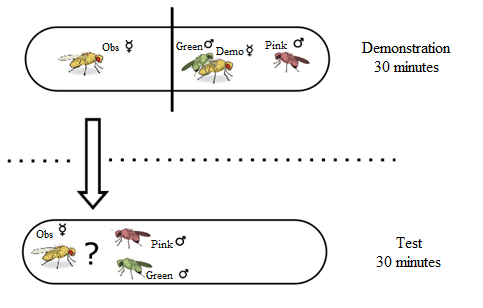
\includegraphics[width=0.8\textwidth]{images/classic}
	\caption{All experimental flies were virgin. During demonstration, observer female observes the free choice of demonstrator female. Observer females are tested immediately after the end of the demonstration. After all copulations ended, demonstrators were removed.}
	\label{fig:Classic protocol}
	\end{figure}

\clearpage

	\subsubsection{Acceptance/Rejection experiment}
	
	During this first experiment, we tested whether mate-copying is achieved through aversive or appetitive memory. To do so, we split the negative and positive information given by the usual mate-copying demonstration. A classical demonstration, in which a demonstrator female chooses between two males, contains a rejection (negative information) of a male and an acceptance (positive information) of the other one. We thus created three demonstration treatments: (1) a control where a demonstrator female freely chooses between two males, (2) an “acceptance” treatment with one accepted male copulating with a demonstrator female, and (3) a rejection treatment with one male actively rejected by a female (Figure 3).
	
		\begin{figure}[h]
		\centering
		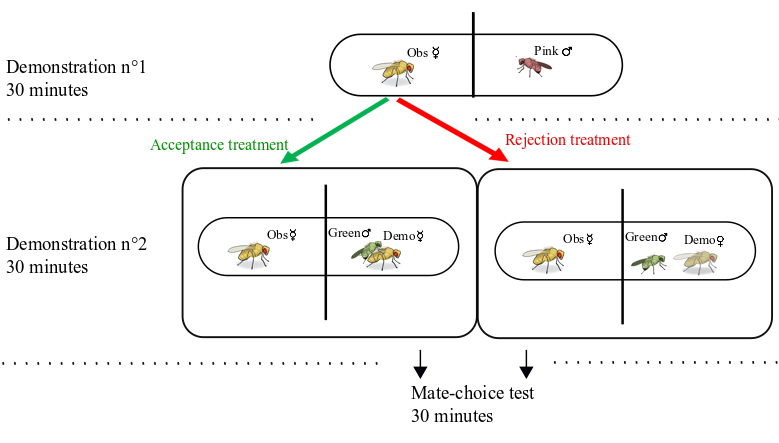
\includegraphics[width=0.8\textwidth]{images/ar}
		\caption{A/R experiment. 
			The demonstration order is reversed each day. For acceptance treatment, both demonstrators were virgin, while for rejection treatment, only males were virgin. For control treatment, the observer female is placed in front of an empty tube for demonstration n°1 and face a free choice of the demonstrator female between two males for demonstration n°2. If the female rejected the male during acceptance treatment, it was switched to rejection and if female accepted the male during rejection treatment, it was switched to acceptance treatment. For each phase, after all copulations ended or 30 minutes, demonstrators were removed.}
		\label{fig:ar}
	\end{figure}
	
	\subsubsection{Neuronal blockade experiment}
	
	This second experiment aimed at exploring the mechanisms underlying the results of the Acceptance/Rejection experiment by discovering one group of dopaminergic neurons involved in mate-copying.
	
	The demonstration was similar to classical protocol (Figure 1), but we used Ddc-GAL4/w+;;UAS-Shits/+ (treatment “Ddc”) and w+/w-;;UAS-Shits/TH-GAL4 mutants (treatment “Gal4”) as observer females. The use of these mutants allowed us to have a temporal control on specific sets of neurons presumably involved in appetitive (Ddc) or aversive (TH) memory, thanks to the thermosensitive activation of Shibire. During the demonstration and 30 minutes before, observer mutant females were heated to a restrictive temperature of 33°C, thanks to a heating mat under the tube of these females. At 33°C, Shibire protein blocks the neurons in which it is expressed, and thus the acquisition of appetitive memory should be blocked in observer females of “Ddc” treatment, and the acquisition of aversive memory in “TH” females. 
	
	After all copulations ended, demonstrator males and females were removed. Observer females were then stored individually in clean tubes at 25°C for 3-4 hours to ensure that labelled neurons are no more blocked, then we proceeded to a classical test at 25°C.


	\subsection{Mate-copying score}

	As in previous studies \parencite{danchin_cultural_2018,nobel_mate-copying_2018,monier_dopamine_2018}, a mate-copying score evaluated female’s tendency to copy the choice of the demonstrator. A mate-copying score of 1 was assigned to females that copulated with the color preferred by demonstrator females and a score of 0 in the opposite case. For each treatment, a mate-copying index was calculated as the mean of mate-copying scores per treatment, a random choice indicated by a value of 0.5. All replicates where only one male courted the female before copulation were discarded because in these situations the female was not unambiguously in a position to make a choice between the two colors.

	\subsection{Statistical analyses}

	All statistical analyses were performed with the R software version 3.5.1 (R Core Team, 2018).
	For each treatment, the difference from a random choice was tested with a binomial test. Mate-copying scores were then analyzed in a generalized linear mixed model (GLMM, package lme4 \parencite{bates_fitting_2015}). Starting models contained the following fixed effects: treatment, normalized air pressure (air pressure in Toulouse-Blagnac weather station, at the time of the beginning of the experiment, minus mean air pressure), normalized air pressure variation within the six preceding hours and all interaction between these three variables, experimenter effect and its interaction with treatment. A random “block” effect was also introduced in the models to account for the non-independence of observer flies from the same block of 6 tubes-set up trained and tested in parallel. The significance of fixed effects was tested using Wald chi-square tests included in ANOVA function (car package, \textcite{fox_r_2018} ). Model simplification was achieved by successive withdrawal of the non-significant terms in a backward selection approach, using P-values and starting with the highest-order interaction. The final model was chosen as the one with the lowest Akaike Information Criteria (AIC, Akaike, 1969). Comparisons between treatments were done using post-hoc X² tests. 
	
	\subsection{Verification of labeled neurons in TH-GAL4 mutants}
	
	In view of the results of the neuronal blockade experiment, we wanted to check the neurons labeled by GAL4 in flies Ddc-GAL4/w+;;UAS-Shits/+. No verification has been conducted so far for this strain, contrarily to TH-GAL4 strain ( Isabel,G Per. Com.).
	
	We crossed
	
	\subsection{Ethical statements}

	Behavioral observations of D. melanogaster required no ethical approval and complied with French laws regarding animal welfare. We kept the number of flies used in this study as small as possible. We handled flies by gentle aspiration without anesthesia to minimize damage and discomfort. After the experiments, individuals were euthanized in a freezer at -20°C.

	\section{Results}

	\subsection{A/R Experiment}
	\label{subsec:AR-experiment}

	For this experiment, we tested 850 females among which 530 copulated during test, including 192 with double-courtship, 64 for each treatment. First we tested for female's color preference with binomial test but neither in the demonstration (N = 850, 426 females copulated with green males and 424 copulated with pink males; binomial test: P = 0.973) nor the test (N = 530, 270 copulated with green and 260 with pink males; binomial test: P = 0.696) was there any significant difference between the two colors.

	For each treatment, the difference from random choice was tested with a binomial test, ``acceptance'' (where the observer female sees a copulation, N = 64, P {\textless} 0.001) and ``control'' (N = 64, P = 0.03) were both significantly different from random, but ``rejection'' treatment (where the observer female sees a male rejected without copulation, N = 64, P = 0.382) was not (Figure 4).

	To test for the significance of mate copying among treatments, we built a global model including the effects of experimenter, treatment, normalized air pressure (actual air pressure minus global mean of air pressure), normalized air pressure variation (for the last six hours) and the interaction between air pressure and variation of air pressure. The selected model included the effect of treatment, air pressure, variation of air pressure and the interaction between air pressure and its variation. Only the treatment had a significant effect on mate-copying (GLMM, $\chi^2$: $N = 192$, $\chi^2 = 10.447$, $p = 0.005$), air pressure (GLMM, $\chi $²: N = 192, $\chi $² = 0.572, p = 0.449) and variation of air pressure (GLMM $\chi $²: N = 192, $\chi $² = 1.831, p = 0.176) were non-significant. The interaction between air pressure and variation of air pressure was close to be significant (GLMM $\chi $²: N = 192, $\chi $² = 2.946, p = 0.086), as we could have expected in regard of the results of \textcite{dagaeff_drosophila_2016}. No significant difference has been found between ``control'' and ``acceptance'' treatments ($\chi $² = 1.76, P = 0.18; Fig4), but both are different from ``rejection'' treatment (acceptance - rejection: $\chi $² = 11.62, P {\textless} 0.005; control - rejection: $\chi $² = 4.52, P = 0.033; Fig4).
	
	\clearpage
		\begin{figure}
		\centering
		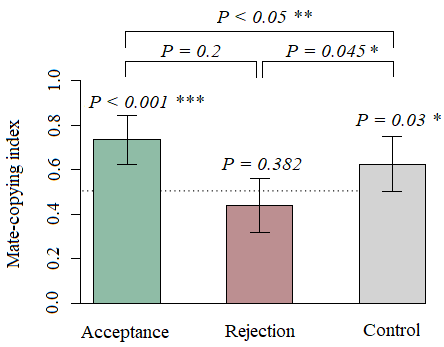
\includegraphics[width=0.8\textwidth]{images/mcsar}
		\caption{Mate-copying index A/R experiment. Mate-copying index is calculated as the mean of mate-copying scores for each treatment. Just above the bars: binomial tests of departure from random choice, ***P<0.005, **P<0.01, *P<0.05, NS P>0.05. Two by two comparisons: post-hoc chi-square tests. Test between all groups: GLMM. Dashed lines indicate random choice, numbers inside the bars represent the sample size.}
		\label{fig:mcsar}
	\end{figure}
\clearpage

\subsection{Neuronal blockade experiment}

For this second experiment, we tested 336 females, among which 208 copulated, including 88 with double courtship. Female's color preference was tested with a binomial test, but we found no preference between the two colors in demonstrations (N = 336, 151 females copulated with green males and 185 copulated with pink males; binomial test: p {\textless}0.072) and tests (N = 208, 107 copulated with green and 101 with pink males; binomial test: p {\textless}0.729).

As for the previous experiment, we first tested difference from random choice for each treatment with a binomial test: females from ``Ddc'' treatment exhibited a mate-copying score different from random (N = 39, p {\textless} 0.024) while ``TH'' did not (N = 49, p {\textless} 0.568)(Fig 5).

To test for the effect of treatment on mate-copying efficiency, we built a global model, including the effects of experimenter, treatment, normalized air pressure (actual air pressure minus global mean of air pressure), normalized air pressure variation (for the last six hours) and the interaction between air pressure and variation of air pressure. The selected model included the effect of treatment, air pressure, variation of air pressure and the interaction between air pressure and its variation.Again, only the treatment had a significant effect on mate-copying (GLMM, $\chi^2$: $N = 88$, $\chi^2 = 4.245$, $p = 0.0394$), while effect of air pressure, variation of air pressure and interaction between air pressure and air pressure variation were non-significant (GLMM, $\chi^2$: $N = 88$, $\chi^2$ = $0.619$, $0.259$ and $2.176$ respectively, $p = 0.4315$, $0.611$ and $0.14$ respectively)(Fig 4).

\clearpage




\begin{figure}
	\centering
	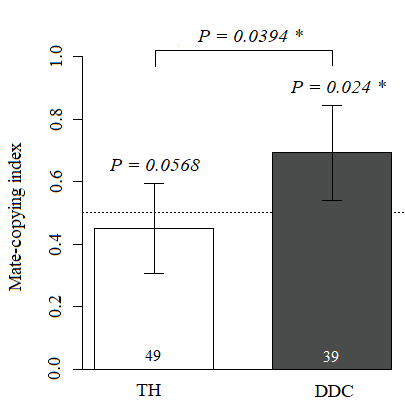
\includegraphics[width=0.8\textwidth]{images/mcnb}
	\caption{Mate-copying index of neuronal blockade experiment. Mate-copying index is calculated as the mean of mate-copying scores for each treatment. Just above the bars: binomial tests of departure from random choice, ***P<0.005, **P<0.01, *P<0.05, NS P>0.05. Test between the groups: GLMM. Dashed lines indicate random choice, numbers inside the bars represent the sample size.}
	\label{fig:mcsar}
\end{figure}

\clearpage
	


\section{Discussion}

So far, mate-copying studies in \textit{Drosophila melanogaster} were based on the acceptance or rejection of different phenotypes by a demonstrator.
Here we showed that the acceptance, not the rejection, of a single male is sufficient to induce mate-copying in females. 
When a female witnessed an acceptance of male followed by a copulation, she exhibited mate-copying. 
In the other case, when observer female witnessed only a rejection of the male, her subsequent choices was similar to random. 
In both cases, only a part of the information was available for the female; but it seems that only positive information matter for mate-copying, since mate-copying index of rejection treatment was not different from random.
%voir papier alvargues  pour interprétation?
Yet, several studies in fish have demonstrated mate-copying without copulation between demonstrators, but they are hardly comparable to our study. 
In theses studies, it was not the copulation that witnessed the choice of the observer female but only the fact that she spends more time with one male than with the other\parencite{dugatkin_lee_alan_reversal_1992,galef_mate-choice_1998}. 
Notably, a study on lekking birds (\textit{Terao tetrix})  showed that females exhibited mate-copying only when the males were able to copulate with demonstrator females. Our results go in the same direction but again, mate-copying was not a matter of biased copulation but of biased attraction to preferred males. In our study, both demonstration and test involved copulation and so it leave little doubt about interpretation. 
The fact that mate-copying relies on acceptance and positive information rather than rejection and negative information is plausible in regard of evolution.
Females can reject copulation for numerous individual-specific reasons. For example, in flies a female can reject a male if she recently mated \parencite{chapman_sex_2003} or if she saw the male copulated recently \parencite{loyau_when_2012}.
In this case, the reason for rejection is pointless for other females and uninformative about the male quality, which is potentially excellent.
Whereas for acceptance, both individual specificities and quality of the male led to the copulation and so acceptance is much more informative.
%Nevertheless, the mate-choice is based on many factors, 
However, we used non-virgin demonstrator females in rejection experiment, and males can smell that the female has recently mated \parencite{jallon_few_1984}. 
Even though we made sure the male actively courted the female, it is possible that his behavior was different because of this smell and that the female observer sees it. 
Its inclination to copy may be impacted, leading to the observed results. 
This point demand further investigation.

Once we knew on what kind of stimulus the mate-copying was based on, we looked at the underlying neuronal mechanisms. 
Surprisingly, we found that TH-labbeled neurons are required in mate-copying, while Ddc neurons are not. 
When heated to a restrictive temperature, Ddc-GAL4 females copied the choice of the demonstrator despite the fact that Ddc neurons was silenced; while in the same context, females with TH-GAL4 neurons silenced didn't exhibited mate-copying, with a similar to random. Yet, we ran out of time and we could not do a control treatment to check if the flies w+/w-;;UAS-Shits/TH-GAL4 had a mate-copying score different from the random. It is possible that the presence of the transgenes impair the functioning of the brain and prevent learning even when the flies are not heated to restrictive temperature. Potentially the incapacity to learn of these flies would not come from the silencing of these neurons but from a more global neural problem due to the use of mutants.
Except the results of \textcite{monier_dopamine_2018}, no study have investigated the neuronal basis of mate-copying in flies. But concerning the formation of appetitive and aversive memory in non-social (direct) learning, the results are antagonistic; TH was responsible of aversive memory and Ddc of appetitive memory. Since our results show that mate-copying is based on appetitive memory, we were expecting Ddc neurons to be required in mate-copying, but we were wrong.
According to our results, TH neurons are required in formation of both aversive direct memory and appetitive indirect memory. 
Thus direct and indirect learning involves different group of neurons. 
And it seems that
Comparable results have been found very recently in rats. \textcite{carrillo_emotional_2018} showed that a specific group of neurons (in Anterior cingulate cortex) responded to a social aversive stimulus (conspecific's pain) but not to an aversive non-social stimulus (a fear-conditioned sound). After deactivation of theses neurons, observer rat showed reduced distress when witnessing pain of conspecifics but freezing in response to fear-conditioned sound was unchanged.
Similarly to our study, these results show that response to social and non-social stimulus involves different group of neurons. Even if it's comparable to our study nature of stimulus and difference in brain structure makes it difficult to draw solid conclusions. But such results potentially underlie the high similarity of learning mechanisms between flies and rat, and more generally mammals. It's especially interesting because \textit{Drosophila melanogaster} is a non-social insect, and the existence of culture in such species make it possible to potentially understand how it evolved throughout the brain's complexification; by studying these neuronal mechanisms in social insects and then in species with more and more complex brains.

In conclusion, we showed that mate-copying in flies comes from the observation of copulation between conspecifics and that it's neuronal pathway is different from those involved in direct associate learning. If several issues temper our conclusions (lack control and use of mated females) 
it does not prevent our results from showing that even after one century spent studying it, much remains to be learned from Drosophila. Future studies should investigate other neuronal structures involved in mate-copying
they allow to dive deeper into the exploration of brain mechanisms, looking for what other neural groups of mushroom body are involved.
In regard of evolution, our results, even if preliminary, are truly interesting as they support the fact that appearance of social cognition did not appear at the same time as the non-social  during life's evolution. 
Moreover, it is relevant from an adaptive point of view  to process differently personal and social stimuli as the issues and the appropriate response are very different. Meanwhile, personal stimuli, even if they come from different sensory cues, conveys information specific to the individual; possible responses are more determined by the valence (positive or negative) of the stimuli than by the fact that it is visual or olfactory(smelling and seeing a predator should lead to similar reactions).
Finally, despite huge differences in brain size and complexity, homology between flies and mammals have led to major advances in our understanding of human neural mechanisms and diseases; specially autism that comes from a problem of neuronal structure related to social cognition. 
More generally, now that mate-copying and a form of animal culture have been shown in flies it is time to understand the neuronal basis of cultural transmission whose importance in the evolution of species is increasingly recognized \parencite{danchin_public_2004}.
Our study is one step further in this direction. 










\clearpage
\newrefcontext[sorting=nyt] % sorts the bibliography by name first, then year, title
\printbibliography
 \end{document}
